\documentclass[a4paper,11pt,stu]{apa}


% Set double spacing
\usepackage{setspace}

% Set captions
\usepackage[
    format=plain,
    font=normalsize,
    labelfont=bf,
    textfont=it,
    labelsep=newline]{caption}
\captionsetup{
    justification=raggedright,
    singlelinecheck=false,
    margin=0cm
    } % Align left
%\AtEveryCite{\normalfont} % Prevent italic anywhere else in the document
\usepackage[capposition=top]{floatrow} % For ``Note.'' underneath the figures
%\DeclareCaptionFont{normal}{\fontsize{11}{13.2}\selectfont}
%\newcommand{\fignote}[1]{\floatsetup{font=normal,cappositon=bottom}\floatfoot{\large \textit{Note.} #1}}

\usepackage{tikz}
\usetikzlibrary{automata,shapes,arrows,calc,positioning,decorations.pathmorphing}

\begin{document}

\begin{figure}[!h]
    \caption{Modelling Academic Records that are Missing not at Random (MNAR) Using Diggle-Kenward Selection Model}
    \label{fig:dk}

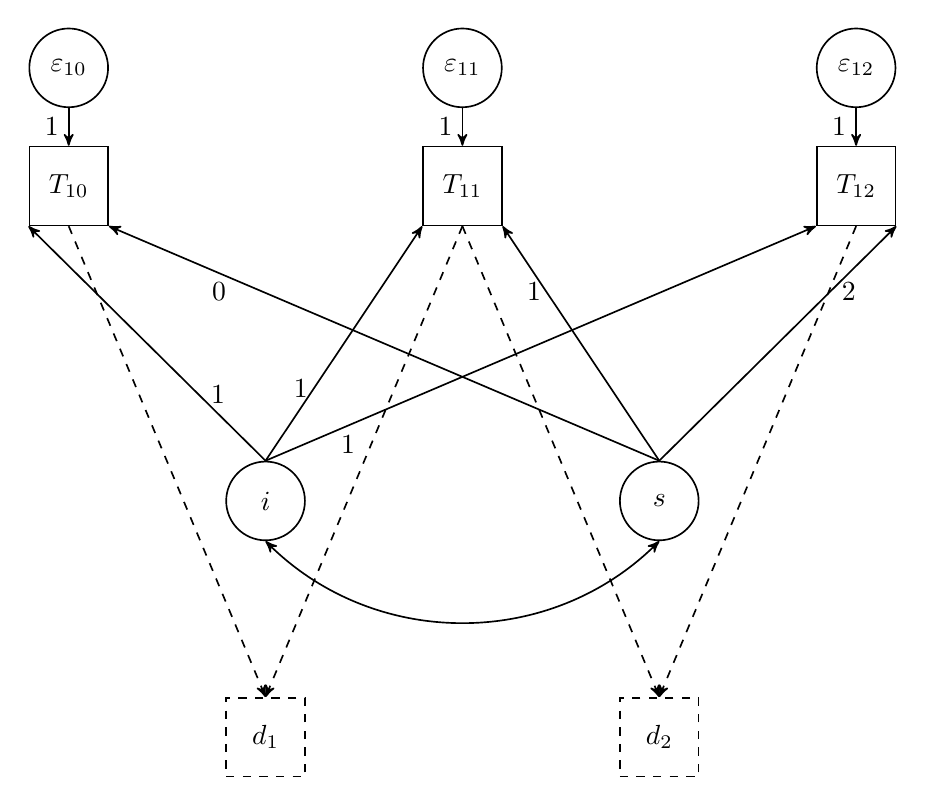
\begin{tikzpicture}[
    latvar/.style={ellipse,draw=black,minimum width=1cm,minimum height=1cm},
    manvar/.style={rectangle,draw=black,minimum width=1cm,minimum height=1cm},
    misvar/.style={dashed,rectangle,draw=black,minimum width=1cm,minimum height=1cm},
    mean/.style={fill=black!10!white,regular polygon,regular polygon sides=3},
    ->,>=stealth',semithick,
    bend angle=-45,
    decoration={
        zigzag,
        amplitude=1pt,
        segment length=1mm,
        post=lineto,
        post length=4pt
    }
]

% Draw missingness (d)
    \node[misvar] (d1) at (2.5,3) {$d_1$};
    \node[misvar] (d2) at (7.5,3) {$d_2$};

% Draw intercept (i) and slope (s)
    \node[latvar] (i) at (2.5,6) {$i$};
    \node[latvar] (s) at (7.5,6) {$s$};

% Draw repeated measures (T)
    \node[manvar] (t1) at (0,10) {$T_{10}$};
    \node[manvar] (t2) at (5,10) {$T_{11}$};
    \node[manvar] (t3) at (10,10) {$T_{12}$};

% Draw residuals (epsilon)
    \node[latvar] (e1) at (0,11.5) {$\varepsilon_{10}$};
    \node[latvar] (e2) at (5,11.5) {$\varepsilon_{11}$};
    \node[latvar] (e3) at (10,11.5) {$\varepsilon_{12}$};

% Link i to T
    \draw[->] (i.north) to node[above,pos=0.2] {$1$} (t1.south west);
    \draw[->] (i.north) to node[above,pos=0.225] {$1$} (t2.south west);
    \draw[->] (i.north) to node[below,pos=0.15] {$1$} (t3.south west);
% Link s to T
    \draw[->] (s.north) to node[below,pos=0.8] {$0$} (t1.south east);
    \draw[->] (s.north) to node[below,pos=0.8] {$1$} (t2.south east);
    \draw[->] (s.north) to node[below,pos=0.8] {$2$} (t3.south east);
% Link epsilon to T
    \draw[->] (e1.south) to node[left] {$1$} (t1.north);
    \draw[->] (e2.south) to node[left] {$1$} (t2.north);
    \draw[->] (e3.south) to node[left] {$1$} (t3.north);
% Allow correlation between i and s
    \draw[<->] (i.south) to [bend left] (s.south);

% Link T to d
    \draw[dashed,->] (t1.south) to (d1.north);
    \draw[dashed,->] (t2.south) to (d1.north);

    \draw[dashed,->] (t2.south) to (d2.north);
    \draw[dashed,->] (t3.south) to (d2.north);

\end{tikzpicture}

    \floatfoot{\normalsize \textit{Note.} Students' academic records in Year 10, 11 and 12 ($T_{10}$ to $T_{12}$) are captured. Solid paths represent latent growth model (LGM) with correlating intercept ($i$) and slope ($s$). Dash lines represent discrete-time survival model for the dropout indicators ($d$).}
\end{figure}

\end{document}